\documentclass[12pt]{article}
\usepackage[margin=1.0in]{geometry}
\usepackage{amsmath}
\usepackage{amsthm}
\usepackage{amsfonts}
\usepackage{amssymb}
\usepackage{latexsym}
\usepackage{graphicx}
\usepackage{listings}
\usepackage{titling}
\usepackage{setspace}
\usepackage[utf8]{inputenc}
\usepackage[english]{babel}
\usepackage{hyperref}
\usepackage{algpseudocode}

\usepackage{xcolor}
\usepackage{listings}
\setcounter{secnumdepth}{4}
\lstset{
    frame=single,
    breaklines=true,
    postbreak=\raisebox{0ex}[0ex][0ex]{\ensuremath{\color{red}\hookrightarrow\space}}
}

\newtheorem{definition}{Definition}[section]
\newtheorem{theorem}{Theorem}[section]
\newtheorem{corollary}{Corollary}[theorem]
\newtheorem{lemma}[theorem]{Lemma}

\sloppy
\setlength{\droptitle}{-1in}
\title{Voice Recognition with Topological Data Analysis}
\author{Joy Patel, Gautam Hathi, Austin Hua}
\date{May 4, 2016}

\begin{document}
\maketitle

\newpage
\tableofcontents

\newpage
\section{Introduction}
\-\hspace{1cm} Our project focuses on the topic of voice discrimination. While
the problem of voice recognition—which involves converting voice to text—is
widely discussed and explored, the problem of distinguishing between
speakers—which we call voice discrimination—is also important. In particular,
there are lots of situations involving new devices such as the Amazon Echo or
Google Home where it is important not only to know what is being said but who
is speaking. Voice discrimination can be a useful tool in these situations.
Current voice technology is very single-user centric, but improving voice
discrimination capabilities opens up a wide range of multi-user applications.
Another possible application is providing another form of biometric security,
potentially allowing users to unlock their phones by voice. These applications
all hinge on improving the accuracy of voice discrimination.
\newline \-\hspace{1cm} In this project, we explore a topological approach to
voice discrimination. We explore different techniques for processing voice
samples that can be used to create good topological features from the voice
data. We then attempt to use a number of machine learning and statistical
techniques to accomplish voice discrimination from topological features, and
compare the results of using topological features vs. non-topological features.

\section{Data}

\-\hspace{1cm} For this project, we collected voice samples from 4 different
people. We had each of these people say the phrase ``open sesame'' 40 times.
``Open sesame'' was chosen because the length of the phrase provided more data
and varied sounds to allow for better discriminatory power than a single word
might provide. A sample refers to a single instance of a single person saying
this phrase. This gave us a dataset with many different people saying the same
phrase, and we could then proceed to try and discriminate between samples in
the dataset from different people. We could then proceed to try and discriminate
between samples in the dataset by the differences in the way people say the
same phrase. Some of the ways these differences manifest themselves are in
pitch, intonation and inflection, and rhythm and cadence. We aim to take
advantage of the effects of these differences by extracting various features as
well as using TDA to compute the degree of similarity between samples.In the
machine learning statistical context, each person is a class. A voice sample is
a signal file, i.e., it can be thought of as a vector in $\mathbb{R}^L$ where
$L$ is the time length of the audio file (sample in 44 kHz).

\section{Process}
\-\hspace{1cm} We explored three components which we put together into a voice
discrimination pipeline.
\begin{figure}[!ht]
\centering
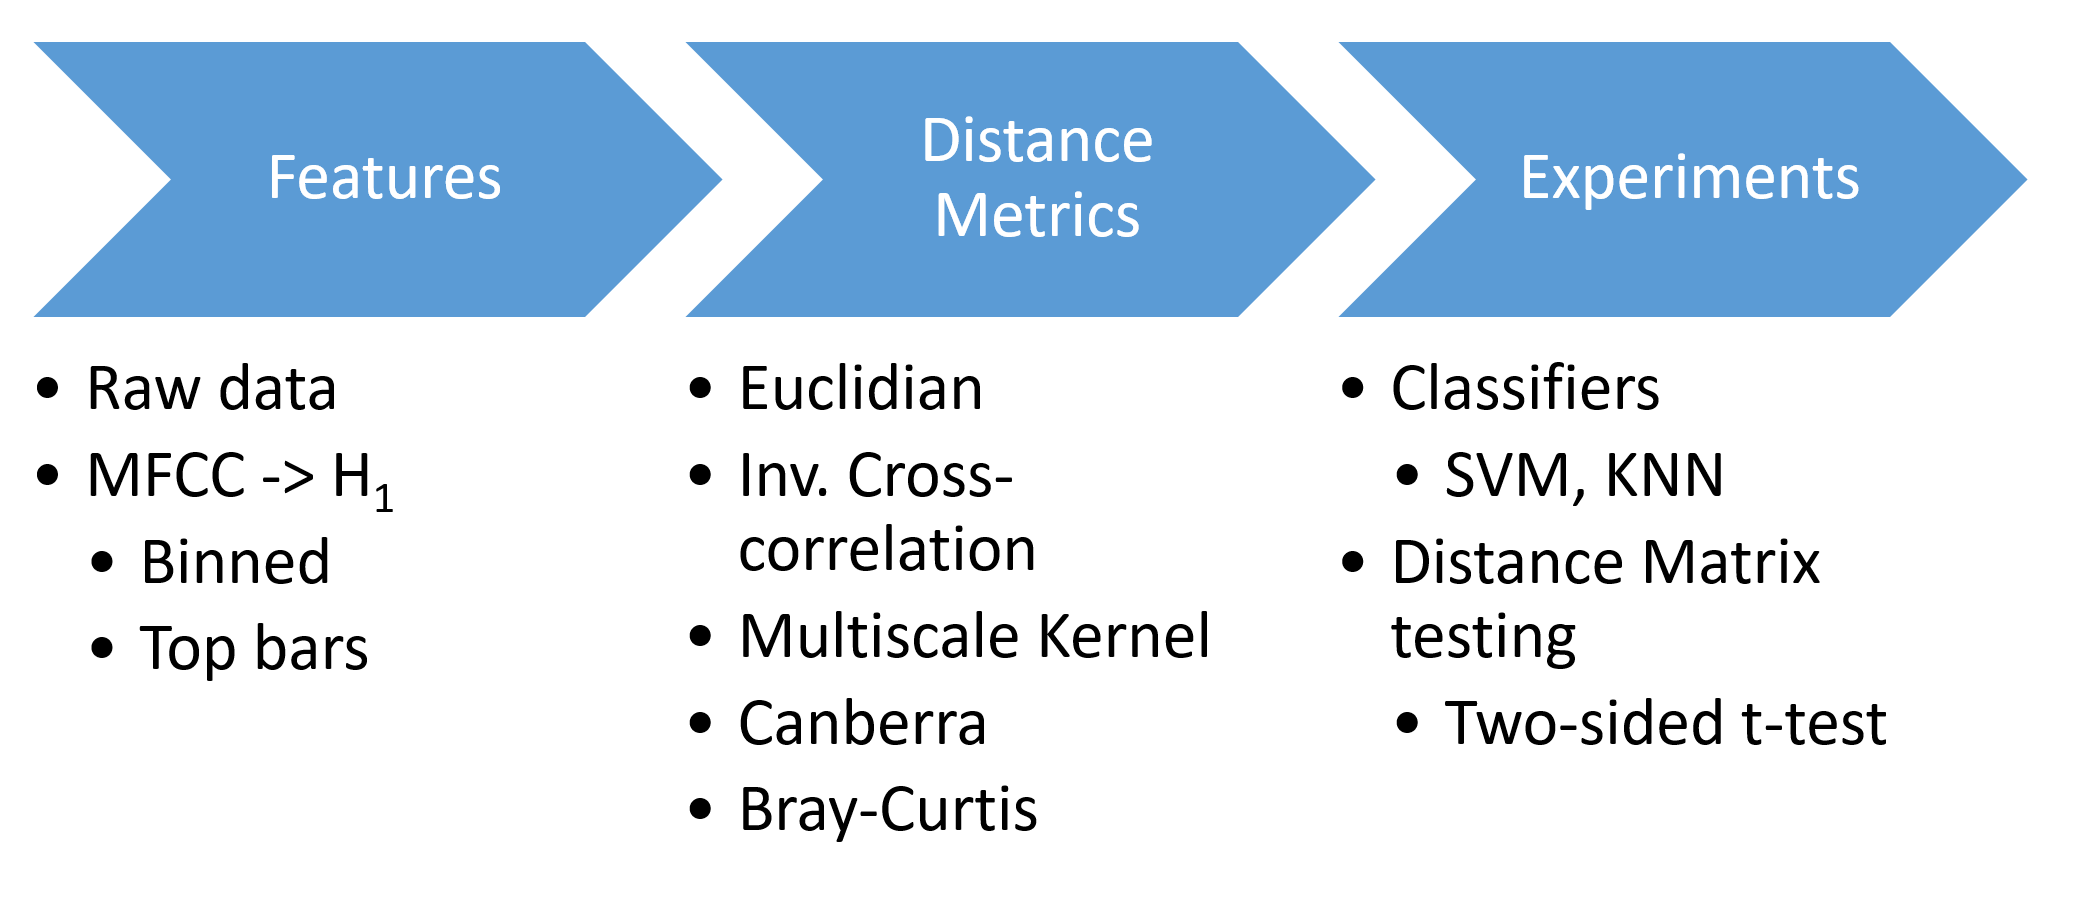
\includegraphics[width=0.8\textwidth]{process.png}
\caption{Process Pipeline}
\end{figure}
\newline
\subsection{Audio Feature Extraction for Topology}
\-\hspace{1cm} We processed each audio sample using a couple of different
feature extraction libraries. To analyze the audio sample topologically, we
computed 1st dimensional homology from these features as well as from the raw
audio data using the Rips complex. From the resulting persistence diagram, we
took the top 10 bars as well as vectors created by binning the persistence
diagram.
\newline \-\hspace{1cm} From the audio data, we compute Mel-Frequency Cepstral
coefficient (MFCC) representation which is time series based on a ``perceptually
motivated log frequency and log power short-time Fourier transform that
preserves timbral information'' \cite{MFCC} \cite{Chris}. MFCC features appeared
to give us the best homology results. The 3rd MFCC coefficient of an audio
sample generally created point clouds with visible cycles in 2D PCA. When we
did TDA on the point cloud, we saw clearly distinguished 1D persistence points
above the diagonal \cite{Chris}:
\begin{figure}[!ht]
\centering
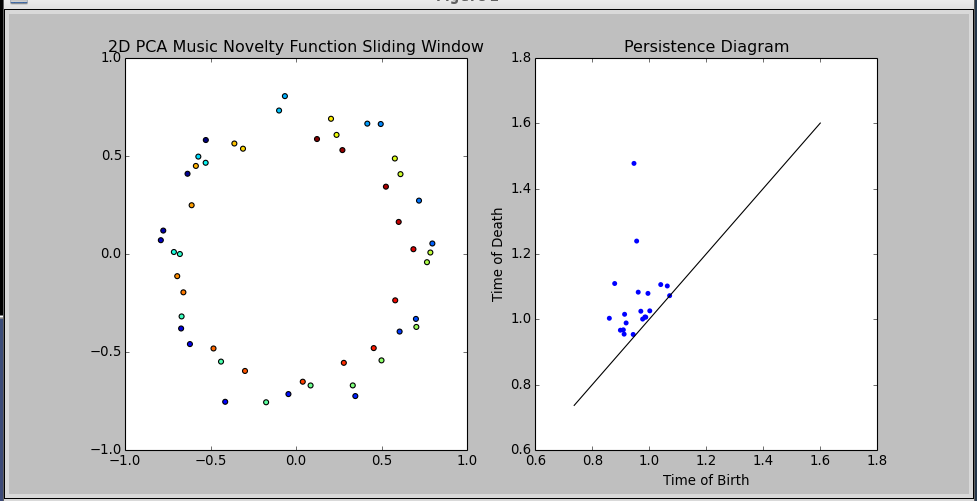
\includegraphics[width=0.8\textwidth]{pd.png}
\caption{1D Homology Persistence Diagram of MFCC Features from Voice Sample}
\end{figure}
\newline \-\hspace{1cm} For subsequent steps in the
process, we used the following features which we generated:
\begin{enumerate}
  \item Persistence Diagram: 1D persistence diagrams generated from sliding
  windows over MFCC features (for use with multi-scale kernel) \cite{Chris}
  \item Top 10 Persistence Bars: Top 10 (death - birth) values from 1D
  persistence diagrams generated from sliding windows over MFCC features (vector
  in $\mathbb{R}^10$)
  \item Binned Persistence Diagrams: Binned 1D persistence diagrams generated
  from sliding windows over MFCC features with 36 bins (vector in
  $\mathbb{R}^36$)
  \item Raw Data: Raw audio sample data (vector in $\mathbb{R}^t$ where t is
  the length of the audio file)
\end{enumerate}


\subsection{Distance Metrics}
\-\hspace{1cm} We explored several different distance heurstics and metrics for
statistical comparisons and classification. Take note of their inputs, that is,
they are metrics and heuristics between different types of features, e.g.,
integer valued vectors, real valued vectors, signal functions, and persistence
diagrams.
\begin{enumerate}
  \item Real Valued Vector Spaces Euclidean Metric \newline $d : \mathbb{R}^n
  \times \mathbb{R}^n \rightarrow \mathbb{R}$ via $d(u,v) = \sqrt{\sum_{i=1}^{n}(u_i - v_i)^2}$
  \item Integer Valued Vector Spaces Canberra Metric \newline $d : \mathbb{Z}^n
  \times \mathbb{Z}^n \rightarrow \mathbb{R}$ via $d(u,v) = \sum_{i = 1}^{n} \frac{|x_i -
  y_i|}{|x_i| + |y_i|}$ \cite{Distance Metric}
  \item Integer Valued Vectors Spaces Bray-Curtis Metric \newline $d :
  \mathbb{Z}^n \times \mathbb{Z}^n \rightarrow \mathbb{R}$ via $d(u,v) = \frac{\sum_{i = 1}^{n}|x_i
  - y_i|}{\sum_{i = 1}^{n}|x_i + y_i|}$ \cite{Distance Metric} \cite{braycurtis}
  \item Real Valued Signal Inverse Max Cross Correlation \newline $d :
  \mathbb{C}^1 \times \mathbb{C}^1 \rightarrow \mathbb{R}$ via $d(f,g) =
  \frac{1}{\max _{\tau \in (-\infty,+\infty)} (\int _{-\infty}^{+\infty}
  f^{*}(t)g(t+\tau)dt)}$ where $f^{*}$ is the conjugate of $f$ \cite{cross
  correlation}
  \item Persistence Diagram Distance Multiscale Kernel \newline $d : PD \times
  PD \rightarrow \mathbb{R}$ via $d(P,Q) = \frac{1}{8 \pi \sigma} \sum_{p \in
  P, q \in Q}(\exp(-\frac{||p-q||^2}{8 \sigma}) -
  \exp(-\frac{||p-\bar{q}||^2}{8 \sigma}))$ where $||v||$ is the Euclidean
  Metric and if $q = (a,b)$, then $\bar{q} = (b,a)$ (note: $\sigma$ is a
  parameter choice; we use $\sigma = 1.0$) \cite{multiscale kernel}
\end{enumerate}

\subsection{Statistics and Machine Learning}
\-\hspace{1cm} In our research, we wish to experiment with both the predictive
capablities of the distance functions with a variety of features. To
discriminate between voice samples from different people, we put the features
extracted from the samples into statistical tests and  classifiers with a
correspondingly appropriate distance metrics.
\subsubsection{Two Sample T Test}
\-\hspace{1cm} We took sets of feature vectors from voice samples of different
people, calculated distances between pairs of vectors within and pairs of
vectors across sets, and ran a two-sided t-test to determine whether the
distances of vector pairs within a set were statistically distinguishable from
the distances of vector pairs across sets. 
\newline \-\hspace{1cm} More concretely: first choose a feature and a
corresponding distance metric $d$. Let $C_i$ be collection of that feature
for person $i$. So, for instance, if the feature you chose was MFCC binned
persistence diagrams, then $C_i$ would be the set of MFCC binned persistence
diagrams for person $i$. Let $C_j, C_k$ feature from voice samples from 2
different people (i.e., 2 different classes).
For $C_k$ and $C_j$, construct $S_1$ and $S_2$ as follows: $S_1 =
\{d(x,y) : x, y \in C_k, x \neq y\}$ and $S_2 = \{d(x,y): x \in C_k, y \in
C_j\}$. Using $S_1$ and $S_2$, run a two sample t-test. The results of this test
will show whether the feature and distance metric chosen have discriminatory
power.
\subsubsection{Machine Learning Classifiers}
\-\hspace{1cm} We trained machine learning classifiers on feature vectors
extracted from voice samples of people and used the different distance metrics
mentioned above for classification using a 60\% training, 40\% testing split of
the data. We experimented with both binary classification (using 2 labels at a
time) as well as multi-label (4 labels) classification using the following sets
of (feature, metric) pairs: (Binned Persistence Diagrams, Canberra Metric),
(Binned Persistence Diagrams, Bray-Curtis Metric), (Binned Persistence
Diagrams, Euclidean Metric), (Top 10 Persistence Bars, Euclidean Metric), (Raw
Data, Inverse Cross Correlation), (Persistence Diagram, Multiscale Kernel
Metric). For the binary classification, we run each of these (feature, metric)
of all pairwise combinations of the people, compute the ratio of
$\frac{\text{true positive}}{\text{testing size}}$ per combiation, and average
the ratios to get an average true positive ratios. Since we use our own
metrics for distance computation, we need classifiers that are also based in
some space with distance (metrics and heuristics). Thus, our classification
experiments are run using SVM and KNN classifiers.

\section{Results}
\subsection{Two Sample T Test Results}
\-\hspace{1cm} The results for a 2 sample T test are shown below for 2 of the
classes.
\begin{figure}[!ht]
\begin{center}
\begin{tabular}{||c|c|c||}
\hline
(feature, metric) & Test Statistics & P-Value \\ 
\hline 
Binned Persistence Diagrams, Canberra Metric & -21.420 & 9.848e-91 \\ 
\hline
Binned Persistence Diagrams, Bray-Curtis Metric & -7.481 & 1.185e-13 \\
\hline 
Binned Persistence Diagrams, Euclidean Metric & -4.218 & 2.601e-05 \\ 
\hline
Top 10 Persistence Bars, Euclidean Metric & 2.112 & 0.0348 \\
\hline
Raw Data, Inverse Cross Correlation & -0.337 & 0.736 \\
\hline
Persistence Diagram, Multiscale Kernel Metric & -2.405 & 0.016 \\
\hline
\end{tabular}
\end{center}
\caption{Two Sample T-Test Results}
\end{figure}
\newpage
\subsection{Classification Results}
\-\hspace{1cm} The results for binary classification (2 labels) are shown below.
The table shows the average of the true positive ratios across all pairwise
combinations of the classes.
\begin{figure}[!ht]
\begin{center}
\begin{tabular}{||c|c|c||}
\hline
(feature, metric) & SVM & KNN \\ 
\hline 
Binned Persistence Diagrams, Canberra Metric & 0.140625 & 0.8125 \\ 
\hline
Binned Persistence Diagrams, Bray-Curtis Metric & 0.21875 & 0.78125 \\
\hline 
Binned Persistence Diagrams, Euclidean Metric & 0.36458333 & 0.77604167 \\ 
\hline
Top 10 Persistence Bars, Euclidean Metric & 0.48958333 & 0.53645833 \\
\hline
Raw Data, Inverse Cross Correlation & 0.42708333 & 0.71875 \\
\hline
Persistence Diagram, Multiscale Kernel Metric & 0.57291667 & 0.5 \\
\hline
\end{tabular}
\end{center}
\caption{Binary Classification Average Results}
\end{figure}
\newline \-\hspace{1cm} The true positive ratio results for multi-label
classification (4 labels) are shown below.
\begin{figure}[!ht]
\begin{center}
\begin{tabular}{||c|c|c||}
\hline
(feature, metric) & SVM & KNN \\ 
\hline 
Binned Persistence Diagrams, Canberra Metric & 0.0 & 0.5625 \\ 
\hline
Binned Persistence Diagrams, Bray-Curtis Metric & 0.046875 & 0.546875 \\
\hline 
Binned Persistence Diagrams, Euclidean Metric & 0.078125 & 0.515625 \\ 
\hline
Top 10 Persistence Bars, Euclidean Metric & 0.265625 & 0.15625 \\
\hline
Raw Data, Inverse Cross Correlation & 0.296875 & 0.59375 \\
\hline
Persistence Diagram, Multiscale Kernel Metric & 0.3125 & 0.25 \\
\hline
\end{tabular}
\end{center}
\caption{4 Multi-Label Classification Results}
\end{figure}
	
\subsection{Discussion}
\-\hspace{1cm} In our discussion of the results, we mainly aim to see how
topological features compared with the raw cross-correlation
(non-topological) feature. We first conducted the two sample T-Tests. The two
sample T-Test clearly shows significance at a 1\% alpha level for the (feature,
metric) pairs involving the Binned Persistence Diagrams feature while showing a
very high p-value for the Raw Data. This gave us reason to believe that
topological tools may be useful for machine learning and are worth
investigating.
\newline \-\hspace{1cm} Afterward, we conducted the machine learning
classification experiments, e.g., experiments that may demonstrate how our voice
recognition might be used in real world applications. For the binary
classification, we found that our best voice discrimination pipeline used
(Binned Persistence Diagrams, Canberra Metric) and a KNN classifier with a true
positive ratio of 0.8125. Using this pipeline, we were able to achieve better
classification results than with (Raw Data, Inverse Cross Correlation) which
had a 0.71875 ratio. Our tests also showed that groups of voice samples
processed with these features were statistically distinguishable. This means
that topological features are promising for voice discrimination purposes with
regard to binary classification. 
\newline \-\hspace{1cm} For the multi-label classification, the (Raw
Data, Inverse Cross Correlation) with 0.59375 ratio ended up outpeforming the
topological features. However, the best topological pair was (Binned
Persistence Diagrams, Canberra Metric) with a close 0.5625 ratio so even though
the Raw Data did better, it was not by a large margin. 
\newline \-\hspace{1cm} We note that the KNN classifier performed better than
the SVM classifier. This indicates that the data we fed into the classifiers
may not have been linearly separable, even under the different distance metrics
we used.

\section{Conclusion}
\-\hspace{1cm} Overall, our experiments demonstrate that topological features
have distinguishing power for voice data.
\newline \-\hspace{1cm} There are still some issues to be
resolved in future work. First, parameter tuning is an important step in the
process that must be explored further. We had to experiment with parameters for
the sliding windows in order to ensure that the MFCC feature extraction worked
properly. We also note that binning our persistence diagrams worked well with
the particular number of bins that we used, and it is unclear how much the
number of bins could be varied while still achieving good results.
\newline \-\hspace{1cm} Performance issues are also a significant consideration.
Some of our distance metrics required careful implementation in order to get
any reasonable performance, and the implementations we used may not be scalable
for large datasets. Determining which distance metrics deliver the best
classification results with a scalable implementation would be an important
step towards making TDA-based voice discrimination viable.
\newline \-\hspace{1cm} Finally, while our results are promising, we cannot
classify voice samples with near-certainty, as would be desired for real-world
applications. Classification accuracy would likely be improved with more data.
We had relatively few samples and our models did better with more data. We also
note that while we had good results with binary classification, our results were not as good with multi-class classification, indicating
that our pipeline may be good for applications such as a voice lock, where the
type of discrimination needed is inherently binary (the user in one class,
and everyone else in the other). Future works should aim to build a
multi-level classifier combining aspects for both raw and topological features. 

\newpage
\section{Bibliography}
\begin{thebibliography}{1}

\bibitem{cross correlation}
Bracewell, R. \textit{Pentagram Notation for Cross Correlation} The Fourier
Transform and Its Applications. New York: McGraw-Hill, pp. 46 and 243, 1965.

\bibitem{MFCC}
Bruce P Bogert, Michael JR Healy, and John W Tukey. \textit{The quefrency
alanysis of time series for echoes: Cepstrum, pseudo-autocovariance,
cross-cepstrum and saphe cracking.} In Proceedings of the symposium on time
series analysis, volume 15, 209-243, 1963. Web. 4 May. 2017.

\bibitem{Chris}
Chirstopher J Tralie and Paul Bendich. \textit{Cover Song Identification with
Timbral Shape Sequences} July 21, 2015. Web. 4 May. 2017.
\url{https://arxiv.org/pdf/1507.05143.pdf}

\bibitem{multiscale kernel}
Reininghaus Jan, Huber Stefan, Bauer Ulrich, Kwitt Roland. \textit{A Stable
Multi-Scale Kernel for Topological Machine Learning} Dec 21, 2014. Web. 4 May.
2017. \url{https://arxiv.org/pdf/1412.6821.pdf}

\bibitem{Distance Metrics}
Scikit-learn Developers. \textit{Sklearn neighbors DistanceMetric}
Sklearn neighbors DistanceMetric-Scikit-learn Documentation. N.p., 2016.
Web. 04 May 2017.
\url{http://scikit-learn.org/stable/modules/generated/sklearn.neighbors.DistanceMetric.html}

\bibitem{braycurtis}
Scipy community. \textit{scipy spatial distance braycurtis} scipy spatial
distance braycurtis Documentation. N.p., 2016. Web. 04 May 2017
\url{https://docs.scipy.org/doc/scipy-0.19.0/reference/generated/scipy.spatial.distance.braycurtis.html}

\end{thebibliography}

\end{document}